\documentclass[11pt]{article}

% ================================================================ packages
\usepackage[margin=1in]{geometry}
\usepackage{amsmath,amssymb,amsthm,mathtools}
\usepackage{graphicx}
\usepackage{booktabs}
\usepackage{microtype}
\usepackage[numbers,sort&compress]{natbib}
\usepackage{xcolor}
\usepackage[colorlinks=true,linkcolor=blue!60!black,citecolor=blue!60!black,urlcolor=blue!60!black]{hyperref}

% ================================================================ theorem envs
\newtheorem{theorem}{Theorem}
\newtheorem{lemma}{Lemma}
\newtheorem{corollary}{Corollary}
\newtheorem{proposition}{Proposition}
\newtheorem{assumption}{Assumption}
\theoremstyle{remark}
\newtheorem{remark}{Remark}

% ================================================================ macros
\newcommand{\kb}{\bar\kappa}
\newcommand{\eps}{\varepsilon}
\newcommand{\epshat}{\hat\varepsilon}
\newcommand{\R}{\mathbb{R}}
\newcommand{\E}{\mathbb{E}}
\newcommand{\Var}{\mathrm{Var}}
\newcommand{\Cov}{\mathrm{Cov}}
\newcommand{\dist}{\mathrm{dist}}
\newcommand{\Phidet}{\Phi_{\mathrm{det}}}
\newcommand{\sigsq}{\sigma^2}

\title{\bf Model Collapse on Manifolds:\\ a Closed-Form Capacity Floor and a Data-Anchoring Fix}
\author{Naman Chandwani\\ \small Independent Researcher\\ \small \texttt{namanchandwani.10@gmail.com}}
\date{July 2026}

\begin{document}
\maketitle

% ================================================================ abstract
\begin{abstract}
Generative models are increasingly retrained on data that includes their own past outputs,
and for diffusion models this \emph{self-consuming} loop is known to degrade quality from
one generation to the next. We settle the case that matters most in practice and that the
sharpest prior theory \citep{khelifa2026recursive} repairs only for smooth densities and
explicitly leaves open---data concentrated on a thin low-dimensional manifold---with
matching negative and constructive results. \emph{Negatively}, we prove a closed-form
\emph{capacity floor}: any truncated reverse-SDE sampler whose normal score slope is capped
at $\kb$ retains excess width of at least $1/(8\kb^2)$ on every pass, with no dependence on
the sampling schedule. The mechanism is geometric: near a manifold of width $\sigma$ the
score a diffusion model must represent is steep only inside a short, finite window of noise
levels, so a slope-capped network bakes in excess width there that later denoising cannot
remove. A model held at a fixed slope ceiling therefore collapses without bound as the manifold
thins, and staying bounded requires a slope budget growing like $\sqrt{J}$ in the Fisher
information $J$. Throughout, the hypothesis bounds the network's normal Lipschitz norm, not
its parameter count; the link from architecture size to attainable slope is measured here,
not proved. Empirically
the trap is two-horned: the
stochastic sampler sticks $\sim\!11\times$ too wide, while the deterministic one collapses to
a point; neither reaches the data. \emph{Constructively}, we prove that periodically
re-matching the model's output to a small, \emph{fixed} pool of real examples makes the loop
\emph{memoryless}, so that error stops compounding for every positive fraction of real data.
The match rescales the output to the \emph{local width} of the reference; it does not
re-insert the reference examples into training. Over a 20-generation head-to-head the
prior state of the art plateaus at $9.8\sigma^2$ while anchoring holds $1.01\sigma^2$, and
on pixel-space MNIST anchoring removes $\sim$81\% of the off-manifold collapse. A
preliminary scale-up to CIFAR-10 in raw pixel space ($3{,}072$ dimensions), across three
seeds, reproduces the separation and, by three independent nearest-neighbor metrics, shows
the anchor keeps full coverage of the real data, ruling out mode collapse. The core
experiments run on CPU and all are reproducible from released scripts.
\end{abstract}

% ================================================================ 1 intro
\section{Introduction}\label{sec:intro}

\paragraph{In plain terms.} Train an image generator, use it to make pictures, then train
the next generator partly on those pictures, and repeat. Each round the model drifts a
little further from real data, the way a photocopy of a photocopy loses detail. This is
\emph{model collapse}. Recent theory shows the drift can be repaired when the data is
``smooth,'' but leaves open the case that actually describes images, audio, and most real
data: points that lie on a thin surface (a \emph{manifold}) inside a much larger space.
This paper handles that case. We prove there is a hard floor on how faithful a
fixed-size model can stay, set by a single number, how sharp an edge the network can
represent, that no amount of tuning removes. Then we give a cheap fix: each round, gently
rescale the model's output so its fine-scale spread matches a small, fixed sample of real
data. The fix stops the drift from compounding, for any positive amount of fresh real data.

Web-scale corpora already contain machine-generated data, and synthetic data is used
deliberately in modern training pipelines. When a generative model is repeatedly
retrained on a pool containing its own previous outputs, quality degrades across
generations, a phenomenon called \emph{model collapse}
\citep{shumailov2024nature,alemohammad2024mad,bertrand2024stability,dohmatob2024tale}.
For diffusion models, \citet{khelifa2026recursive} give the sharpest analysis to date:
with a fraction $\lambda$ of fresh real data per generation and an annealed truncation
schedule $t_0(g)\to0$, the recursion converges back to the data distribution,
\emph{provided the data has finite Fisher information} (their Case~1). They explicitly
leave open their Case~2: data supported on, or concentrated near, a low-dimensional
manifold, where the Fisher information $J\asymp(d-k)/\sigsq$ diverges as the noise width
$\sigma\to0$. Essentially all natural data (images, audio, molecular conformations) is
of this second kind \citep{fefferman2016testing,pidstrigach2022manifold}.

This paper answers Case~2.

\paragraph{The idea in one paragraph.} The hardest property to preserve across generations
is the data's \emph{thinness}---the exact width of a pen stroke, the sharp edge of a shape.
A finite-capacity denoiser can reproduce that thinness only inside a brief window of noise
levels, so a small, fixed amount of blur is baked in every generation and accumulates. This
yields our two results, made precise below: a \emph{negative} one---the blur has an exact
floor set by a single number, the steepest slope the network can represent, that no training
or sampling schedule lowers---and a \emph{constructive} one---the accumulation is cancelled
by periodically re-matching the model's output to the \emph{local width} of a small,
unchanging set of real examples, without copying those examples back into training.

\textbf{The negative half} is a \emph{capacity floor} (Section~\ref{sec:floor}). The
score that a diffusion model must represent near a $\sigma$-thin manifold has normal
slope $\kappa(t)=s(t)/\gamma^2(t)$ which is \emph{non-monotone} in diffusion time: it
peaks at $\kappa_{\max}=1/(2\sigma)$ near $t\approx\sigsq$ and falls back toward zero as
$t\to0$ (Figure~\ref{fig:mechanism}a). A network whose normal slope is bounded by $\kb$
therefore under-contracts on a \emph{finite band} of diffusion times; the excess variance
frozen in while crossing that band can never be removed afterwards, because too few
contraction e-folds remain below the band. We prove that in the singular limit the
resulting floor is a universal function of the single ratio $\rho=\kb/\kappa_{\max}$ and
admits \emph{closed forms}: under no assumption beyond the slope bound, the floor is
exactly $\sigsq/(2\rho^2)=1/(8\kb^2)$, so a fixed network collapses relatively without
bound as $\sigma\to0$, and bounded collapse requires $\kb=\Omega(1/\sigma)=\Omega(\sqrt J)$.
No truncation schedule enters these statements: annealing targets a term the schedule can
kill, while the floor lives in a term it cannot touch. Empirically the trap is
\emph{two-horned} (Figure~\ref{fig:trap}): keeping the reverse-SDE noise, the sampler
sticks $\sim\!11\times$ too wide; removing it, the recursion collapses to a single point.
Neither branch reaches the data.

\textbf{The constructive half} is an anchoring operator (Section~\ref{sec:fix}). A
bidirectional, per-axis, local moment match of the training pool (and sampler output) to
a small \emph{stale} reference of real data (2{,}000 samples drawn once at generation
zero) pins the normal variance at the reference value each generation. We prove this
makes the recursion \emph{memoryless}: the fixed-point equation loses its dependence on
the previous generation, the critical fraction disappears, and the dynamics of
\citet{khelifa2026recursive}'s Theorem~4.1 are restored in the singular regime. In a
20-generation head-to-head against their annealed-truncation remedy
(Figure~\ref{fig:headtohead}), the annealed arm plateaus at $9.8\sigma^2$ while the
anchored arms hold $1.01\sigma^2$, flat, on both samplers we test; on real pixels
(MNIST), anchoring closes $\sim$81\% of the collapse gap (Figure~\ref{fig:mnist}); and a
preliminary CIFAR-10 pixel recursion ($3{,}072$ dimensions, three seeds) reproduces the
anchored/unanchored split with full mode coverage (Figure~\ref{fig:cifar}).

\paragraph{Contributions.}
\begin{enumerate}\itemsep2pt
\item \textbf{A law of collapse} (Theorem~\ref{thm:law}): under a measured
  one-dimensional concave response law, the variance recursion has a unique plateau for
  $\lambda>\lambda^*=c_\infty/(1+c_\infty)$ and no plateau below; truncation enters only
  additively, which makes precise why annealing schedules cannot help singular data.
\item \textbf{A closed-form capacity floor} (Theorem~\ref{thm:floor},
  Corollary~\ref{cor:capacity}): any reverse-SDE sampler with normal score slope
  $\le\kb$ is floored; in the singular limit the floor is $1/(8\kb^2)$ unconditionally
  and $\big((1+3e^{-4})/8\big)\kb^{-2}$ for the empirically observed no-overshoot class:
  two constants that differ by only $5.5\%$. Bounded relative collapse as $\sigma\to0$
  requires $\kb\ge 1/(2\sigma\sqrt{2C})$.
\item \textbf{A memorylessness theorem for anchoring} (Theorem~\ref{thm:fix}): matching
  pool and output normal variance to a stale real reference removes the recursion's
  memory, for every $\lambda>0$, with an error bound independent of the ambient dimension.
\item \textbf{Falsifiable empirics}, each targeting a named claim:
  \begin{itemize}\itemsep1pt
  \item \emph{Floor anatomy \& intervention}: the law's envelope explains ${\sim}60\%$ of
    the measured single-pass floor, the remainder resolving into two further measured
    channels (in-band profile sag; ensemble displacement); and across five training
    protocols that move the ceiling $3.5\to7.5$, every measured floor stays above its
    proven bound.
  \item \emph{Two-horned ablation}: separates the floor's existence (sampler noise) from
    its size (slope ceiling).
  \item \emph{Head-to-head}: a 20-generation, 5-seed win over the state-of-the-art remedy,
    with a replay-buffer control at the anchor's exact information budget that separates
    anchoring from replay, and a subcritical-fraction run exhibiting the law's no-plateau
    regime.
  \item \emph{Real and scaled data}: a pixel-space MNIST recursion, and a preliminary
    CIFAR-10 pixel recursion (three seeds) that rules out mode collapse by three
    independent nearest-neighbor metrics.
  \end{itemize}
\end{enumerate}

Throughout we keep the epistemic status of each claim explicit: \emph{we prove}
(mathematics, given stated assumptions), \emph{we observe} (multi-seed experiments), or
\emph{we model} (measured structural laws that we do not derive). Section~\ref{sec:limits}
collects everything in the third category.

% ================================================================ 2 related
\section{Related work}\label{sec:related}

\textbf{Model collapse.} Collapse under recursive training is documented and analyzed
across model families
\citep{shumailov2024nature,alemohammad2024mad,dohmatob2024tale,bertrand2024stability,gerstgrasser2024collapse};
accumulation (rather than replacement) of data and sufficient fresh-data fractions
mitigate it in the absolutely continuous setting. \citet{khelifa2026quantifying} bound
error propagation in recursively trained diffusions via a discounted accumulation
argument, but their assumptions require absolutely continuous data (structurally
excluding manifolds), with fixed truncation and upper bounds rather than laws.
\citet{khelifa2026recursive} characterize the limiting collapse distribution spectrally
and prove annealed truncation converges for finite-Fisher data (their Case~1), stating
manifold-supported data (Case~2) as open. We give the Case~2 answer: a floor theorem for
their sampler class, and an operator restoring their Case~1 dynamics.

\textbf{Diffusion on manifold data.} That diffusion models detect and concentrate on
data manifolds is established \citep{pidstrigach2022manifold,debortoli2022convergence}.
The singular ($\sigma\to0$) score is the object of a growing one-shot literature: optimal
denoising under low regularity \citep{beyler2025optimal}, provable learning under the
manifold hypothesis \citep{huang2026provable}, and mitigation of the score singularity
\citep{liu2025euclidean}. These works are one-generation; our subject is the
\emph{recursion}, where a per-generation floor compounds into a permanently displaced
plateau. We use the Tweedie/posterior-mean jump \citep{efron2011tweedie,beyler2025optimal}
as a raw-error reducer inside the loop and are explicit that it does not, by itself,
break the floor (Section~\ref{sec:fix}).

\textbf{Local geometry estimation.} Our anchoring operator estimates local tangent
frames by $k$NN-PCA; its error analysis imports standard local-PCA perturbation rates
\citep{aamari2019nonasymptotic,singer2012vector}. The operator needs only \emph{shared}
frames between pool and reference, not correct ones, which is why these rates enter
only at second order (Lemma~\ref{lem:frames}).

% ================================================================ 3 setup
\section{Setup}\label{sec:setup}

\paragraph{Data model ($\sigma$-tube).} Let $M\subset\R^d$ be a compact smooth
$k$-dimensional manifold with reach $\tau>0$. Data are
$X_0=\varphi(U)+\sigma N_\perp$, with $U$ uniform on $M$ and $N_\perp$ standard normal in
the $(d-k)$-dimensional normal space; $\sigma>0$ is the tube width. The singular regime
is $\sigma\to0$; the Fisher information of the marginal scales as
$J\asymp(d-k)/\sigsq\to\infty$ (Case~2 of \citealp{khelifa2026recursive}).

\paragraph{Forward process and the normal coordinate.} We use the
variance-preserving OU forward process $X_t=a(t)X_0+s(t)Z$ with $a(t)=e^{-t/2}$,
$s^2(t)=1-e^{-t}$ \citep{ho2020ddpm,song2021sde}. Fix a point of $M$ and work in a
normal coordinate $x\in\R$, treating the fiber marginal as Gaussian and decoupled from
tangential position (\emph{flat-tube idealization}; curvature enters at $O(s^2/\tau)$
and is tracked where it matters). Then
$X_0\sim\mathcal N(0,\sigsq)$, $X_t\sim\mathcal N(0,\gamma^2(t))$ with
$\gamma^2=a^2\sigsq+s^2$, and the denoising target is linear:
\begin{equation}
\eps^*(x,t)=\kappa(t)\,x,\qquad
\kappa(t)=\frac{s(t)}{\gamma^2(t)},\qquad
\nabla\log p_t(x)=-\frac{x}{\gamma^2(t)} .
\label{eq:kappa}
\end{equation}
$\kappa$ is the normal slope the score network must represent. It satisfies
$\kappa\approx1/s$ for $s^2\gg\sigsq$, peaks at $\kappa_{\max}=1/(2\sigma)$ near
$t\approx\sigsq$, and falls back to $0$ as $t\to0$ (Figure~\ref{fig:mechanism}a). In the
singular limit the \emph{peak} slope diverges, which is the precise sense in which infinite
Fisher information bites the estimator.

\paragraph{Samplers.} $S_{\mathrm{trunc}}(t_0)$ integrates the learned reverse SDE
from $T$ down to $t_0>0$ (Euler-Maruyama,
$x\leftarrow x+(-\tfrac12x+\epshat/s)\,dt+\sqrt{|dt|}\,\xi$) and outputs $x_{t_0}$; all
prior remedies, including the annealed schedules of \citet{khelifa2026recursive}, are of
this class. $S_{\mathrm{jump}}(\hat t)$ integrates only to a moderate $\hat t$ and then
outputs the Tweedie posterior-mean jump
$\hat x_0=(x_{\hat t}-s(\hat t)\,\epshat)/a(\hat t)$
\citep{efron2011tweedie,beyler2025optimal}.

\paragraph{The recursion.} For a distribution $p$ on $\R^d$ define the per-direction
normal second moment $v(p)=\E_p[\dist(X,M)^2]/(d-k)$; true data has $v=\sigsq$.
Generation $g$ trains $\epshat_g$ by denoising score matching on
$\mathrm{pool}_g=\lambda\,(\text{fresh real})+(1-\lambda)\,(\text{generation }g\!-\!1)$
and samples; $v_g$ is the output value. Since $v$ is linear in the measure,
$w_g:=v(\mathrm{pool}_g)=\lambda\sigsq+(1-\lambda)v_{g-1}$ exactly.

\paragraph{Modeling assumptions (\emph{we model}).} Our law rests on two assumptions
about the trained pipeline that we \emph{measure and cross-validate} but do not derive.

\begin{assumption}[scalar reduction]\label{ass:a0}
The per-generation map factors through the pool width: $v_g=F_g(w_g)$.
\emph{Why a scalar:} the collapse observable is a \emph{variance} along the normal
fibre, one number per normal axis by construction, so this is an order-parameter
statement (the width closes on itself) rather than a claim that the network is scalar, in
the same way an order parameter closes a mean-field recursion without the microscopic state
being low-dimensional.
\emph{Validation:} fixed points measured in one experiment type predict those of an
independent type within $1$ to $13\%$ across six $(t_0,\lambda)$ cells
(Section~\ref{sec:experiments}).
\end{assumption}

\begin{assumption}[concave response]\label{ass:a2}
$F_g(w)=a^2(t_0(g))\,w+s^2(t_0(g))+e^2(w)$, where the sampling excess
$e^2:[0,\infty)\to(0,\infty)$ is nondecreasing and concave with $e^2(0)=e_0^2>0$.
\emph{In words:} the output width is the pool width shrunk by the forward map
($a^2w$), plus the truncation remainder ($s^2$), plus a sampler-added excess $e^2$
that (i) never vanishes even for a perfectly thin pool ($e_0^2>0$, this is the floor),
(ii) grows with a fatter pool but (iii) with diminishing returns (concave: doubling the
pool width less than doubles the added excess).
\emph{Why concave:} the excess comes from the network failing to represent the steep part
of the score, and a fatter pool is \emph{easier} to represent (the required peak slope
$\kappa_{\max}=1/(2\sigma_{\text{pool}})$ falls), so each extra unit of pool width buys
less extra error, exactly a saturating (concave) response.
\emph{Validation:} two independent estimators. The direct probe (training
single-width pools and measuring $dv/dw-1$; Appendix~\ref{app:details}) gives a local
slope that is small and nonincreasing, $+0.13\to+0.05$, across the upper half of the
measured range, where all of the recursion's fixed points sit; its small magnitude is
itself a measured near-cancellation of two $O(0.7)$ channels
(Section~\ref{sec:experiments}). The recursion's own local convergence rates give an
independent, indirect estimate that falls from $+0.6$ at the thinnest measured
fixed-point pool ($\lambda=0.75$) to $\approx0$ at the fattest ($\lambda=0.25$): the
same saturating direction, though the two estimators disagree in magnitude where they
overlap, and we treat the rate-based values as directional only (rate fits must
separate a transient, a known failure mode of that estimator). At the probe's thinnest
widths the slope estimates rise from $0$, a regime the recursion never visits; the
law's conclusions require only a unique downcrossing of $T(v)-v$, which the measured
slopes ($\le0.13$ at every fixed point, against thresholds
$\lambda/(1-\lambda)\ge1/3$ at every plateau-forming fraction we test, $\lambda\ge1/4$)
guarantee.
\end{assumption}

% ================================================================ 4 law
\section{The law of collapse}\label{sec:law}

Under Assumptions~\ref{ass:a0} and~\ref{ass:a2} the recursion is one-dimensional:
\begin{equation}
v_g=T(v_{g-1})+s^2_g,\qquad
T(v)=\lambda\sigsq+(1-\lambda)v+e^2\!\big(\lambda\sigsq+(1-\lambda)v\big),
\label{eq:recursion}
\end{equation}
with $s^2_g:=s^2(t_0(g))$ the truncation remainder. (The display takes $a^2(t_0)=1$;
the general case replaces $s^2_g$ by $\eta_g=s^2_g+(a^2(t_0(g))-1)w_g$. Its second
term $\to0$ as $t_0\to0$ whenever $w_g$ stays bounded (part i), and at the small fixed
$t_0$ we use it is $O(t_0 w_g)$, absorbed into the fitted law; in the divergent case
(part ii) we work with the display form, where $\eta_g=s^2_g\ge0$ only strengthens the
conclusion.) Let
$c_\infty:=\lim_{w\to\infty}e^{2\prime}(w)$ (exists by concavity) and define the
\emph{critical real-data fraction} $\lambda^*:=c_\infty/(1+c_\infty)$.

\emph{How to read the theorem.} The per-generation update $T$ pushes the width toward a
balance point. Part (i): if you keep enough fresh real data ($\lambda>\lambda^*$) there is
a single stable plateau the width always settles to, from any start and any schedule.
Part (ii): below that fresh-data threshold there is no plateau at all, the width runs off
to infinity. (For our trained pipeline the measured saturated slope puts $\lambda^*$ at
$\approx0.03$--$0.05$; Section~\ref{sec:experiments} locates it and exhibits both
regimes.) Part (iii): if the sampler excess happens to be a straight line in the pool
width, the plateau has a clean closed form. The one thing to notice is what $\lambda^*$
and $v_\infty$ depend on: the sampler excess $e^2$, \emph{not} the truncation schedule,
which is the whole point of Remark~\ref{rem:annealing}.

\begin{theorem}[law of the collapse; \emph{we prove}]\label{thm:law}
Fix $\lambda\in(0,1]$.
\textbf{(i)} If $\lambda>\lambda^*$, $T$ has a unique fixed point $v_\infty>0$ solving
$v=\lambda\sigsq+(1-\lambda)v+e^2(\lambda\sigsq+(1-\lambda)v)$, and for every $v_0\ge0$
and every truncation schedule with $s_g^2\to0$ the iterates converge, $v_g\to v_\infty$,
with local rate $\rho_{\mathrm{loc}}=(1-\lambda)\big(1+e^{2\prime}(w_\infty)\big)<1$
(where $w_\infty=\lambda\sigsq+(1-\lambda)v_\infty$ is the fixed-point pool width; the
strict inequality is forced by $T(0)>0$, Appendix~\ref{app:law}).
\textbf{(ii)} If $(1-\lambda)(1+c_\infty)>1$, then $T(v)-v\ge T(0)>0$ for all $v$ and
$v_g\to\infty$: no plateau, for any schedule.
\textbf{(iii)} In the affine special case $e^2(w)=e_0^2+cw$:
$\lambda^*=c/(1+c)$, $\rho_{\mathrm{loc}}=(1+c)(1-\lambda)$, and
$v_\infty=\big((1+c)\lambda\sigsq+e_0^2\big)/\big(\lambda(1+c)-c\big)$.
\end{theorem}

\begin{proof}
Appendix~\ref{app:law}. Elementary but complete: concavity gives a unique downcrossing
of $T(v)-v$; contraction above the fixed point plus a monotone barrier below give
convergence under vanishing perturbations.
\end{proof}

\begin{remark}[why annealing cannot help singular data]\label{rem:annealing}
Truncation enters \eqref{eq:recursion} only through the additive, schedule-killable
$s^2_g$. The plateau $v_\infty$ is determined by $e^2$ alone, which no schedule touches.
The remedy of \citet{khelifa2026recursive} is the special case $e^2\equiv0$ (their
Case~1 assumptions make the estimation term schedule-dominated), where indeed
$v_\infty=\sigsq$. Case~2 is precisely the regime where $e^2$ has a floor, the subject
of the next section.
\end{remark}

% ================================================================ 5 floor
\section{The capacity floor}\label{sec:floor}

\begin{figure}[t]
\centering
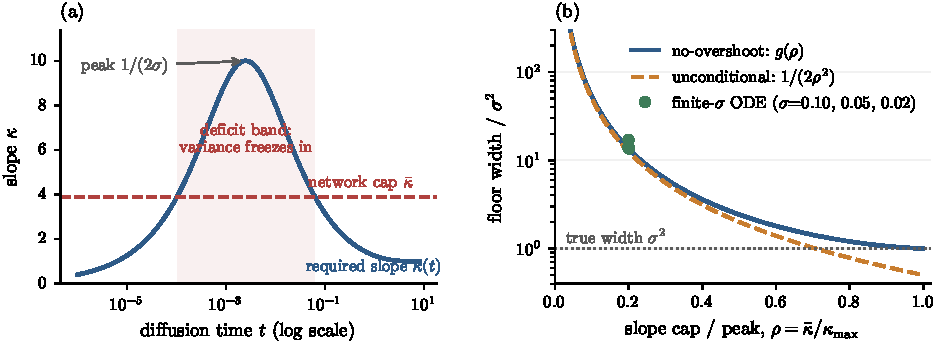
\includegraphics[width=\linewidth]{figs/fig0_mechanism.pdf}
\caption{\textbf{The mechanism and the law.} (a) The required normal slope
$\kappa(t)=s/\gamma^2$ is non-monotone: it peaks at $\kappa_{\max}=1/(2\sigma)$ near
$t\approx\sigsq$ and falls back to zero. A network with ceiling $\kb<\kappa_{\max}$
under-contracts only on a \emph{finite band} (shaded, the cap-to-curve deficit lens);
variance frozen in the band cannot be removed below it (too few contraction e-folds
remain). (b) The resulting floor in units of $\sigsq$ as a function of $\rho=2\sigma\kb$:
closed-form no-overshoot law $g(\rho)$ (blue, Theorem~\ref{thm:floor}), exact
unconditional law $1/(2\rho^2)$ (orange). Green rings: direct finite-$\sigma$ ODE
integration at $\sigma=0.05$ swept across $\rho$ (self-checked against the appendix
triples), sitting just above $g(\rho)$ and following the no-overshoot branch, the
relative $O(\sigsq/\rho^2)$ convergence the theorem predicts. The dotted vertical marks
$\rho=1/\sqrt2$, below which the floor exceeds the true width $\sigsq$.}
\label{fig:mechanism}
\end{figure}

We now prove that for manifold data the sampling excess $e^2$ of any truncated
reverse-SDE sampler is floored by the normal slope its $\eps$-predictor realises. No
decomposition of the network is required. Let $X_t$ be the sampler's \emph{own} ensemble at
noise level $t$ and define the \emph{realised normal slope}
\begin{equation}
\hat\kappa(t)\;:=\;\frac{\Cov\big(X_t,\,\epshat(X_t,t)\big)}{\Var(X_t)},
\label{eq:khat}
\end{equation}
the $L^2$ regression slope of the estimator on the normal coordinate under the law the
sampler actually visits. For an affine estimator this is its slope; for an arbitrary
nonlinear one it is the only functional of $\epshat$ that the variance flow can see.
The structural fact behind the floor (proof in Appendix~\ref{app:ode}):

\begin{lemma}[variance ODE; \emph{we prove}, exact]\label{lem:ode}
Under the reverse Euler scheme, for an \emph{arbitrary} estimator $\epshat$ and with
$\hat\kappa$ as in \eqref{eq:khat}, the ensemble normal variance obeys, in the small-step
limit,
\begin{equation}
-\frac{dV}{dt}=\Big(1-\frac{2\hat\kappa(t)}{s(t)}\Big)V+1 .
\label{eq:varode}
\end{equation}
With the exact slope $\hat\kappa=\kappa$, $V(t)=\gamma^2(t)$ solves \eqref{eq:varode}
exactly. The forcing $+1$ is the sampler's own injected noise. No linearisation is
performed: to first order in the step a single Euler step moves the variance only through
$\Cov(X,\epshat(X))$, the $O(dt^2)$ remainder vanishing in the limit; equivalently, in
continuous time It\^o's formula yields \eqref{eq:varode} directly, with no expansion.
\end{lemma}

\begin{remark}[a checkable sufficient condition]\label{rem:lip}
The hypothesis of Theorem~\ref{thm:floor} constrains $\hat\kappa$, a regression slope. A
pointwise bound implies it: if $\epshat(\cdot,t)$ is $\kb$-Lipschitz in the normal
coordinate then, for an i.i.d.\ copy $X'$ of $X_t$,
\[
\Cov\big(X,\epshat(X)\big)=\tfrac12\E\big[(X-X')(\epshat(X)-\epshat(X'))\big]
\le\tfrac{\kb}{2}\E\big[(X-X')^2\big]=\kb\Var(X),
\]
so $\hat\kappa(t)\le\kb$ under \emph{any} law. Lipschitz control is therefore sufficient
but not necessary; we state the theorem on $\hat\kappa$ because it is the weaker hypothesis
and because it is what \eqref{eq:varode} actually contains.
\end{remark}

This is the precise sense in which the floor is \emph{not} an artifact of linearizing the
score. An earlier version of this argument split $\epshat$ into an affine $L^2(p_t)$ fit
plus an orthogonal residual and invoked the normal equations to discard the residual to
first order. That step is no longer needed, and with it goes its one soft spot: the normal
equations hold under $p_t$, whereas the sampler's own ensemble deviates from $p_t$.
Equation \eqref{eq:varode} is exact for the fully nonlinear network precisely because
$\hat\kappa$ is defined under the sampler's law from the outset. The crux is the geometry
of the required slope:

\begin{lemma}[finite band; \emph{we prove}]\label{lem:band}
$\kappa(t)$ rises from $0$, peaks at $\kappa_{\max}=1/(2\sigma)$ at $t\approx\sigsq$,
and falls back to $0$ as $t\to0$. Hence for any ceiling $\kb<\kappa_{\max}$ the deficit
set $\{t:\kappa(t)>\kb\}$ is a finite band; below it the exact slope is representable
again, but only $2\log(1+\rho^2/4)\le\rho^2/2$ contraction e-folds remain
($\rho:=2\sigma\kb$), so variance frozen in the band persists to $t_0\to0$.
\end{lemma}

In the singular limit the whole flow collapses onto a one-parameter family
(Appendix~\ref{app:floor} for proofs and error terms):

\begin{lemma}[singular-limit ODE; \emph{we prove}]\label{lem:limitode}
Rescale $t=\sigsq u$, $V=\sigsq W$, and write the slope envelope as
$\hat\kappa(t)=(1/\sigma)m(u)$ with $m(u)=\rho/2$ (unconditional envelope) or
$m(u)=\min\{\sqrt u/(1+u),\rho/2\}$ (no-overshoot envelope). Then \eqref{eq:varode}
becomes, as $\sigma\to0$ at fixed $\rho$,
\begin{equation}
-\frac{dW}{du}=1-\frac{2m(u)}{\sqrt u}\,W ,
\label{eq:limitode}
\end{equation}
a $\sigma$-free equation; the uncapped equation has exact solution $W=1+u$
(the rescaled true marginal), and deviations contract quadratically under downward
integration. Consequently
$\lim_{t_0\to0}V(t_0)/\sigsq=g_{\mathrm{class}}(\rho)\big(1+O(\sigsq/\rho^2)\big)$
(a \emph{relative} correction: the boundary-layer perturbation scales with the leading
term $W\sim\rho^{-2}$, so the additive gap to $g$ is $O(\sigsq/\rho^4)$, as the
finite-$\sigma$ values confirm):
\textbf{universality in $\rho$ is a theorem}.
\end{lemma}

\emph{How to read the theorem.} There is one dimensionless knob, $\rho=\kb/\kappa_{\max}=
2\sigma\kb$: how close the network's slope ceiling gets to the peak slope the data demands.
The floor is a universal function of $\rho$ alone. Version (U) makes no assumption on the
network and gives the clean bound $1/(8\kb^2)$; version (N) additionally assumes the
network never over-shoots the true slope (which is what we measure) and gives a slightly
tighter constant. The two constants differ by only $5.5\%$, so for intuition either one is
``the'' floor. The single takeaway: when $\rho<1/\sqrt2$ the floor sits strictly above the
true width $\sigsq$, i.e.\ the sampler is stuck too fat, and it gets relatively worse the
thinner the manifold.

\begin{theorem}[closed-form capacity floor; \emph{we prove}]\label{thm:floor}
Let the trained score's normal slope satisfy $\hat\kappa(t)\le\kb<\infty$
(a finite normal Lipschitz constant: a bound on slope, not on parameter count), and set
$\rho=2\sigma\kb$. Then for every truncation time $t_0>0$ and every schedule:

\textbf{(U) Unconditional.} With no further assumption (arbitrary overshoot permitted),
\begin{equation}
V(t_0)\;\ge\;\sigsq\,\frac{1}{2\rho^2}\,(1+o(1))
\;=\;\frac{1}{8\kb^2}\,(1+o(1)) \qquad(\sigma\to0),
\label{eq:uncond}
\end{equation}
where $1/(2\rho^2)$ is the \emph{exact} value of \eqref{eq:limitode} with $m\equiv\rho/2$:
$\;W(0^+)=\int_0^\infty e^{-2\rho\sqrt u}\,du=1/(2\rho^2)$. The floor exceeds $\sigsq$
whenever $\rho<1/\sqrt2$, i.e.\ $\kb<\kappa_{\max}/\sqrt2$.

\textbf{(N) No-overshoot.} If additionally $\hat\kappa(t)\le\kappa(t)$ (the empirically
observed profile; the network never over-contracts), the tighter floor
$V(t_0)\ge\sigsq\,g(\rho)(1+o(1))$ holds with the explicit closed form: writing
$q=\sqrt{1-\rho^2}$, $x_\mp=(1\mp q)/\rho$, $u_\mp=x_\mp^2$,
\begin{equation}
W_{\mathrm{exit}}=(1+u_+)e^{-4q}+\frac{(3-2q)-(3+2q)e^{-4q}}{2\rho^2},
\qquad
g(\rho)=1+\frac{W_{\mathrm{exit}}-(1+u_-)}{(1+u_-)^2} .
\label{eq:closedform}
\end{equation}
$g(\rho)>1$ for every $\rho\in(0,1)$ with $g\to1$ only as $\rho\to1^-$, and
$g(\rho)=C_0/\rho^2+O(1)$ as $\rho\to0$ with $C_0=(1+3e^{-4})/2=0.5275$, i.e.\ the
deterministic single-pass floor $\Phidet:=\lim_{t_0\to0}V(t_0)=\sigsq\,g(\rho)$
satisfies $\Phidet\to\big((1+3e^{-4})/8\big)\kb^{-2}=0.1319\,\kb^{-2}$.

The two asymptotic constants, $1/8$ and $(1+3e^{-4})/8$, differ by $5.5\%$: the class
distinction is quantitatively minor. The closed forms match direct integration of
\eqref{eq:limitode} to $\le2.4\times10^{-5}$ across $\rho\in[0.1,1]$, and the
finite-$\sigma$ ODE converges to them from above at the stated relative
$O(\sigsq/\rho^2)$ rate.
\end{theorem}

\begin{corollary}[$\sigma\to0$: the answer to Case 2; \emph{we prove}]\label{cor:capacity}
Hold $\kb$ fixed and let $\sigma\to0$ ($J\to\infty$). Then unconditionally
$V/\sigsq\ge(1+o(1))/(8\kb^2\sigsq)\to\infty$: a truncated sampler held at a fixed slope
ceiling collapses \emph{relatively} without bound, for every annealing schedule. Conversely,
bounded relative collapse $V/\sigsq\le C$ requires
\begin{equation}
\kb\;\ge\;\frac{1}{2\sigma\sqrt{2C}}\;=\;\Omega(1/\sigma)\;=\;\Omega(\sqrt J).
\end{equation}
Truncated sampling of singular data demands a slope budget growing with the singularity.
This constrains the normal Lipschitz norm: a fixed architecture can meet it only by enlarging
its weights, and whether training in fact does so is the empirical question the $\kb(w)$ probe
addresses. We thank Wei Huang for pressing this distinction.
\end{corollary}

\begin{figure}[t]
\centering
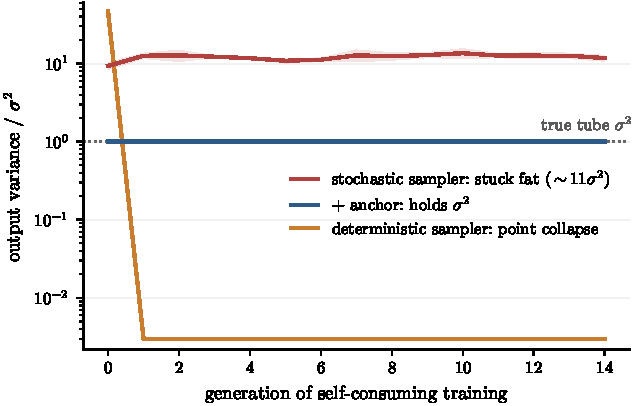
\includegraphics[width=0.72\linewidth]{figs/fig2_two_horned_trap.pdf}
\caption{\textbf{The two-horned trap (\emph{we observe}).} Self-consuming recursions at
fixed $t_0=10^{-4}$, no anchor, 3 seeds. With the reverse-SDE noise on, the recursion
sticks fat at $10.8$ to $13.2\,\sigsq$ (red). With the noise zeroed (deterministic
sampler), it collapses to a \emph{single point} within one generation (orange; verified
loss of all 2-D spread, no numerical overflow). Neither branch reaches the tube
($\sigsq$, dotted); the anchored recursion (blue, Section~\ref{sec:fix}) holds it.}
\label{fig:trap}
\end{figure}

\paragraph{What each ingredient does (\emph{we observe}).} The ablation of
Figure~\ref{fig:trap} separates the roles exactly as \eqref{eq:varode} dictates: the
sampler's own noise (the $+1$) is load-bearing for the floor's \emph{existence}:
switching it off sends $V\to0$ (point collapse, the deterministic horn), while the
finite ceiling $\kb$ makes the floor \emph{larger than} $\sigsq$ (the stochastic horn).
The two branches bracket the target from both sides; no choice of the sampler noise
magnitude attains it.

\paragraph{Confronting the floor with a real network (\emph{we observe}).} For our
standard pipeline the measured slope profile tracks $\kappa(t)$ faithfully at benign
times ($\hat\kappa/\kappa=0.95$ to $0.97$ for $t\ge0.1$) and then saturates at
$\kb\approx3.7$--$4.3$ (seed range) while $\kappa$ continues to $\sim\!10$. The law's
envelope value at the measured ceiling, $\Phidet=3.8$--$4.6\,\sigsq$
(Figure~\ref{fig:floorlaw}), is a \emph{proven lower bound}; the directly measured
single-pass floor at $t_0=10^{-4}$ is $6.3$--$7.5\,\sigsq$, so the bound holds and its
envelope component accounts for $55$--$65\%$ of the measurement, with the exact-score
control reproducing $\gamma^2(t_0)$ to all displayed digits. The remainder is not
mysterious: re-running the sampler's own discrete variance recursion with measured
inputs resolves it into two channels. \textbf{(i) Profile shape}: the measured
$\hat\kappa(t)$ sags $\approx0.5$--$0.7$ below its own ceiling inside the deficit band,
worth $+0.7\,\sigsq$ at the data width. \textbf{(ii) Ensemble displacement}: regressing
the network's normal response on the sampler's \emph{own} ensemble at every step ---
which is fatter than $p_t$ once excess accumulates, so it probes the S-shaped response
into its flattening tails --- gives a smaller effective slope, worth $+2.6\,\sigsq$;
the affine recursion driven by this measured ensemble slope then reproduces the sampler
to $-0.4\,\sigsq$, i.e.\ the nonlinear remainder beyond the two channels is small (this
measures exactly the $\hat\kappa$ of \eqref{eq:khat}, and prices the remaining nonlinear
discrepancy). \textbf{Interventional test.} The law survives moving the ceiling: five
training protocols ($t$-importance-sampling into the band, $4\times$ steps, a
higher-frequency time embedding, and combinations) move $\kb$ from $3.5$ to $7.5$; the
measured floor drops from $7.4$--$7.8\,\sigsq$ at the two low-$\kb$ protocols into the
$2.5$--$4.9\,\sigsq$ range at the three high-$\kb$ ones (a group-level fall with
protocol-dependent scatter, not a clean $1/\kb^2$ trace), and --- the load-bearing
statement --- every one of the five sits strictly above its own proven bound.

\paragraph{What sets the ceiling (\emph{we observe}).} The interventions also identify
the ceiling's origin. Raising the time-embedding frequency alone does nothing
($\kb=3.5$): expressivity in $t$ is not binding. Importance-sampling training times
into the band ($\kb\to6.7$) or simply training $4\times$ longer ($\kb\to6.4$) moves it
strongly: under the uniform $t$-draw the deficit band holds ${<}1\%$ of the training
measure (and $t<10^{-3}$ is never drawn at all, though the sampler visits it), so the
ceiling is \emph{gradient starvation} --- an optimization constant, not an
architectural one, consistent with its independence of sample size and its degradation
on fatter pools (a fatter tube spreads the same starved gradient over an easier, wider
band). The Case-2 conclusion is unchanged --- as $\sigma\to0$ the demanded peak
$1/(2\sigma)$ diverges, so any fixed training budget caps $\kb$ --- but the constant is
steerable: band-weighted noise-level sampling buys a $2$--$3\times$ lower per-pass
floor at fixed size. It cannot reach $\sigsq$, and the recursion compounds whatever
remains, so anchoring is still the fix.

\begin{figure}[t]
\centering
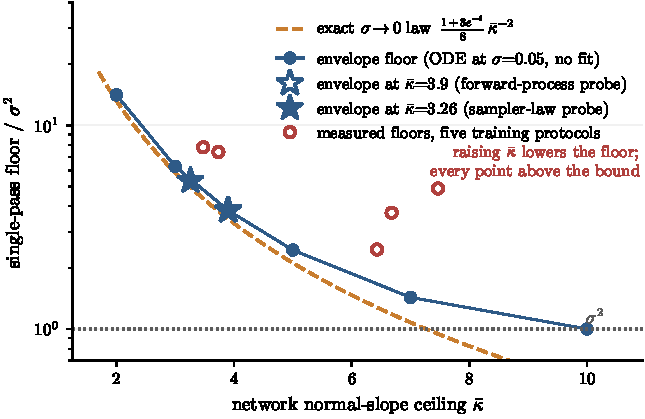
\includegraphics[width=0.7\linewidth]{figs/fig4_capacity_floor.pdf}
\caption{\textbf{The capacity floor: predicted, measured, and moved.} Blue line with
markers: finite-$\sigma$ variance-ODE envelope floor at $\sigma=0.05$ (no fit).
Dashed: the exact $\sigma\to0$ law $\big((1+3e^{-4})/8\big)\kb^{-2}$ of
Theorem~\ref{thm:floor}. Star: the envelope bound $3.8\sigsq$ at the standard
pipeline's measured ceiling $\kb=3.9$ --- a proven lower bound that accounts for
${\sim}60\%$ of the directly measured single-pass floor; the measured anatomy of the
remainder (profile sag, ensemble displacement) is in the text. Open circles: the
interventional test --- five training protocols move the measured ceiling from $3.5$
to $7.5$; the measured floor falls from ${\sim}7.6\,\sigsq$ (low $\kb$) into the
$2.5$--$4.9\,\sigsq$ range (high $\kb$), with protocol scatter, and every point stays
strictly above its bound.}
\label{fig:floorlaw}
\end{figure}

\paragraph{An honest gap, closed in three measured steps (\emph{we model}).} Iterating
the floor through the recursion (every generation's pool is at least as wide as
$\lambda\sigsq+(1-\lambda)\Phidet$) with the network's \emph{clean-tube} ceiling
$\kb=3.9$ gives a deterministic fixed point $v^*_{\mathrm{det}}=4.5\,\sigsq$. The
measured recursion floor is $\approx11\,\sigsq$, a factor $2.4$ above; our theorem
claims only a \emph{lower bound} on the recursion (respected). We account for that
factor in three measured steps, each a directly logged measurement.

\emph{Step 1, capacity degradation.} The single-width probe
(Appendix~\ref{app:details}) shows the ceiling itself degrades on fatter training pools,
from $3.7$--$4.3$ at $\sqrt w=0.03$ down to $2.8$--$3.0$ at $\sqrt w=0.13$ (ranges over
three training seeds), and the degradation replicates under a half-width network, under a
different ring radius (slopes $-9.4$ to $-13.0$ across all five measurements), across
three further synthetic geometries --- a flat segment (the flat-tube idealization made
exact, so the degradation does not require curvature; $42\%$ drop over the same width
range), a sphere in $\R^3$ ($30\%$), and a circle in $\R^{10}$ (codimension 9; $49\%$)
--- and, crucially, on \emph{genuine MNIST $8\times8$ pixel data} (whose digit manifold
has a measured intrinsic normal width $\sigma_0\approx0.072$, thin against its tangent
scale $\approx0.41$): with the identical extraction protocol and per-point $k$NN-PCA
normal frames, $\kb$ falls $2.0\to1.6$ as $\sqrt w$ runs $0.071\to0.231$ ($21\%$),
tightly fit by $\kb(w)\approx2.2-2.7\sqrt w$ (max residual $0.017$, two seeds). The
degradation is therefore not a synthetic-tube artifact. Constants are
geometry-specific. Over this range the points are well described by the
two-parameter fit $\kb(w)\approx4.4-11.6\sqrt{w}$, an \emph{empirical fit, not a derived
form}; nothing below depends on the choice, since refitting linear, logarithmic, or
quadratic, or replacing the fit with a fit-free monotone interpolation of the raw points,
moves the resulting fixed point by at most $10\%$ (the computation uses the fit only as an
interpolant inside the measured range).

\emph{Step 2, the self-consistent closure.} Feeding the degradation back,
$v\leftarrow\Phidet\big(w(v),\kb(w(v))\big)$, moves the fixed point from $4.5$ to
$5.6$--$7.1\,\sigsq$ at $t_0=10^{-4}$ (the range across the three probe seeds' fits), with
the resulting pool width $\sqrt{w^*}\approx0.091$--$0.101$ \emph{inside} the measured
support (interpolation, not extrapolation). The closure assumes the degradation depends on
the pool only through its width $w$, while the recursion's actual pools are two-component
mixtures (clean tube plus fattened returns); testing this directly by training on the fixed
point's own mixture composition gives $\kb^{\mathrm{mix}}=3.37\pm0.15$ against the
single-tube prediction $3.34$, so the width-only reduction survives its first direct test.
This closure shrinks the unexplained factor from $2.4$ to $1.5$--$2.0$ --- a quarter to a
half of the logarithmic gap.

\emph{Step 3, the measured remainder.} For what remains we first say what it is
\emph{not}: iterating the map with the measured generation-to-generation fluctuations gives
a Jensen bias of only $0.006\,\sigsq$, and applying the measured $t\ge0.1$ slope-tracking
ratio ($0.95$--$0.97$) to the whole profile moves the fixed point by only
$+0.3$--$0.4\,\sigsq$. The remainder is then \emph{measured}: the profile-sag and
ensemble-displacement channels of the floor anatomy above, re-measured across six pool
widths spanning the fixed point, lift the per-pass map to its directly measured values, and
iterating that measured map gives a fixed point of $9.9\,\sigsq$ against the measured
$10.8$--$13.2\,\sigsq$ --- the once factor-$2.4$ discrepancy is now $1.1$--$1.3$, at the
level of protocol differences (mixture pools, per-generation sample counts, seed scatter).
What stays underived are the constants themselves: $\kb$, its degradation law, and the
saturation profile.

% ================================================================ 6 fix
\section{The anchoring fix}\label{sec:fix}

\begin{figure}[t]
\centering
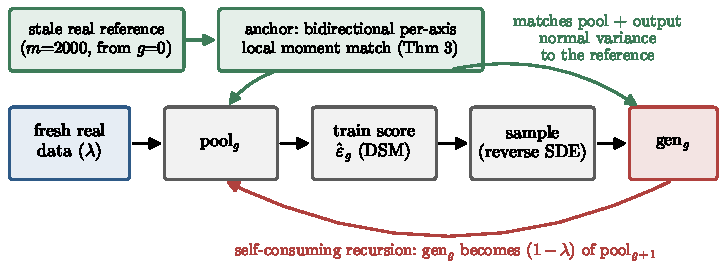
\includegraphics[width=0.95\linewidth]{figs/fig5_pipeline.pdf}
\caption{\textbf{Where the anchor sits.} Each generation, the pool (and, for the jump
pipeline, the sampler output) is passed through a bidirectional per-axis local moment
match against a \emph{stale} reference of $m=2{,}000$ real samples drawn once at $g=0$.
No provenance labels are needed; the reference is never refreshed.}
\label{fig:pipeline}
\end{figure}

Corollary~\ref{cor:capacity} says the singular regime cannot be won by scaling the
model or tuning the schedule. It can be won by \emph{anchoring the recursion to data}.

\paragraph{The operator.} For each point, find its $k$ nearest neighbors in the
reference; take the local PCA frame (top-$k_{\dim}$ directions tangent, remainder
normal); rescale the point's normal coordinates so that the pool's local normal
second moments equal the \emph{reference's} local normal second moments in the
\emph{same estimated frames}. The match is \emph{bidirectional} (it contracts fat
directions and inflates thin ones) and \emph{per-axis}. Both properties are forced by
the theory: the sampler's error is signed (fat from injection, thin from posterior-mean
sharpening; Proposition~\ref{prop:sharpening} in Appendix~\ref{app:sharpening}) and
anisotropic whenever the normal spectrum straddles $s^2(\hat t)$, so any scalar or
one-sided matcher mis-corrects some directions (\emph{we observe}: a scalar matcher
leaves MNIST-latent thin ratios at $0.62$; the per-axis matcher achieves
$|\text{thin}-1|\le0.012$).

\begin{lemma}[shared-frame cancellation; \emph{we prove} to first order]\label{lem:frames}
Let both reference and pool normal energies be measured in the same $k$NN-PCA frames
estimated from the reference. Then the matched pool satisfies, per normal direction,
$v(\mathrm{matched})=\hat\sigma^2_{\mathrm{ref}}+O_p(m^{-1/2})+\Delta_{\mathrm{leak}}$,
where the frame-error leakage $\Delta_{\mathrm{leak}}$ afflicts pool and reference
\emph{identically} at first order in the frame perturbation and cancels; standard
local-PCA rates \citep{aamari2019nonasymptotic,singer2012vector} enter only at second
order. Every quantity in the bound is intrinsic ($k,\tau,\sigma,m$); the ambient
dimension $d$ appears nowhere.
\end{lemma}

\emph{How to read the theorem.} The collapse of Theorem~\ref{thm:law} happens because
generation $g$ inherits generation $g\!-\!1$'s width: the map $F_g$ has a $v_{g-1}$ inside
it, so errors compound. The matcher overwrites the pool's normal width with a fixed number
(the reference's) \emph{before} training, so the input to $F_g$ no longer depends on
$v_{g-1}$. The recursion becomes a constant sequence, there is nothing left to compound,
and the critical-fraction threshold of Theorem~\ref{thm:law} disappears entirely. The only
error left is the one-time cost of estimating the reference width from a finite sample, and
that does not grow with generations.

\begin{theorem}[anchoring makes the recursion memoryless; \emph{we prove} given
Lemma~\ref{lem:frames} and Assumption~\ref{ass:a0}]\label{thm:fix}
Insert the matcher after pooling (and after sampling, for the jump pipeline). Write
$\eps_m:=O_p(m^{-1/2})+\Delta_{\mathrm{leak}}$ for the matcher error of
Lemma~\ref{lem:frames}, a quantity that does not grow with $g$. Then the
training input has normal variance $\hat\sigma^2_{\mathrm{ref}}+\eps_m$
\emph{regardless of $v_{g-1}$}: the map \eqref{eq:recursion} loses its $v$-argument,
\[
v_g=F_g\big(\hat\sigma^2_{\mathrm{ref}}+\eps_m\big),
\]
a constant sequence up to the non-compounding $\eps_m$. Consequently: no fixed-point
equation, \textbf{no critical fraction, and stability for every $\lambda>0$}; and with
$S_{\mathrm{trunc}}$ the dynamics reduce to truncation-only, restoring the
\emph{conclusion} of \citet{khelifa2026recursive}'s Theorem~4.1 in the singular regime
(the data remains singular; what anchoring removes is the compounding term that their
hypotheses excluded).
\end{theorem}

\paragraph{Why this is not a replay buffer.} Replay, data-accumulation, and data-refresh
remedies \citep{gerstgrasser2024collapse,bertrand2024stability} fight collapse by
\emph{re-inserting real examples} into the pool: they preserve \emph{samples}. The anchor
preserves something weaker and more portable, the \emph{local normal moments} (per-axis
widths) of a small stale reference, and imposes them on \emph{whatever the model currently
generates}. It never adds a reference point to the training pool, uses no provenance labels,
and reuses the same $m{=}2{,}000$ points for every generation. The distinction is not
cosmetic. A replay buffer of size $m$ still lets the $(1-\lambda)$ synthetic majority set the
pool's fine-scale statistics, so the floor of Section~\ref{sec:floor} still governs that
majority; anchoring instead \emph{overwrites} the fine-scale statistics of the majority
itself, which is why it removes the floor rather than diluting it. In the language of the law
(Theorem~\ref{thm:law}): replay changes $\lambda$; anchoring changes the response map $F_g$.
We test this at the anchor's exact information budget (\emph{we observe}): inserting the
anchor's own stale reference ($m=2{,}000$ real points, drawn once at $g=0$, never
refreshed) \emph{into the pool} every generation of the head-to-head protocol ---
raising the effective real fraction to $\lambda_{\mathrm{eff}}=2/3$, with synthetic data
now a $1/3$ \emph{minority} --- moves the 20-generation plateau only from $9.8\pm1.7$ to
$8.5\pm1.1\,\sigsq$ (5 seeds, same annealed schedule), the small dilution the law
predicts for a larger $\lambda$; the anchor, using the same $2{,}000$ points as a moment
reference instead, holds $1.01\pm0.02\,\sigsq$. Replay dilutes the floor; anchoring
removes it.

\paragraph{Attribution, stated plainly.} In our pipeline the \emph{matcher} is the
floor-breaker; the Tweedie jump is a \emph{raw-error reducer}. The jump's raw output is
itself fat ($7$ to $20\times\sigsq$ across settings); its value is a $\approx2\times$
smaller one-shot raw error and $\approx3\times$ smaller unanchored plateau
($21$ vs $68\,\sigsq$ in raw normal variance, at $\lambda=\tfrac12$ and matched moderate
truncation $t_0=\hat t=0.05$; the standard plateau includes the truncation remainder
$s^2(0.05)/\lambda\approx39\,\sigsq$ that the jump removes, and the jump plateau is
itself predicted by Theorem~\ref{thm:law} as
$e^2_{\mathrm{jump}}/\lambda$), plus smaller post-match tails. Post-anchor, the standard
and jump samplers converge to the same variance; we report both.

\begin{figure}[t]
\centering
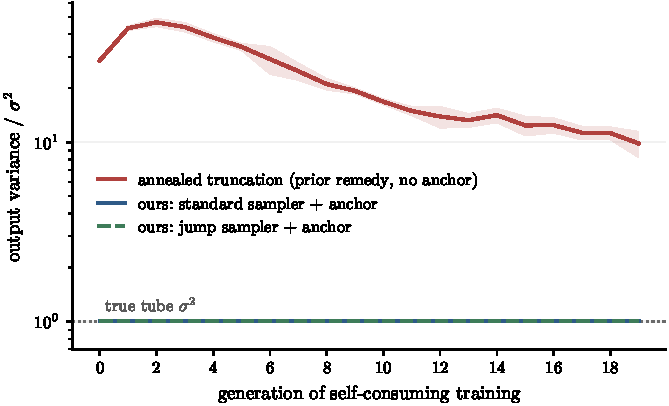
\includegraphics[width=0.78\linewidth]{figs/fig1_head_to_head.pdf}
\caption{\textbf{Head-to-head vs.\ the state-of-the-art remedy (\emph{we observe}).}
Ring manifold, $\sigma=0.05$, $\lambda=\tfrac12$, 20 generations, 5 seeds
(mean $\pm$ s.d.). Red: annealed truncation $t_0\!:0.05\to10^{-4}$, no anchor
\citep{khelifa2026recursive}; it rises to $47\sigsq$, then thins only to
$9.8\sigsq\pm1.7$. Blue/green: the same recursion with the anchor (standard and jump
samplers): $1.01\sigsq\pm0.02$, flat for 20 generations.}
\label{fig:headtohead}
\end{figure}

\begin{figure}[t]
\centering
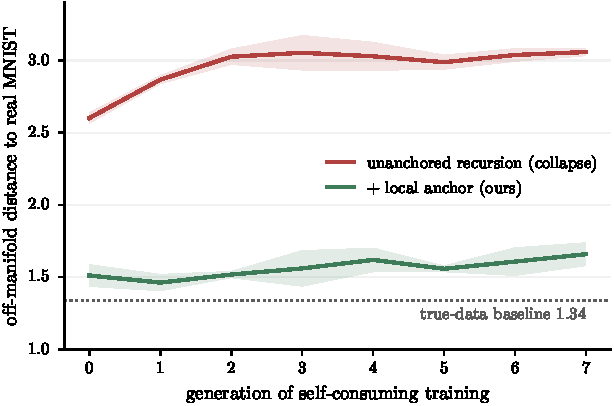
\includegraphics[width=0.72\linewidth]{figs/fig3_pixel_mnist.pdf}
\caption{\textbf{Real pixels (\emph{we observe}).} Self-consuming recursion on
$8\times8$ MNIST (64-dimensional pixel space), $\lambda=\tfrac12$, 8 generations,
3 seeds. Off-manifold distance = mean nearest-neighbor distance to a held-out real test
set. Unanchored drifts to $3.06$ ($2.3\times$ the true-data baseline $1.34$); anchored
holds $1.66$ ($1.24\times$), closing $\sim$81\% of the gap. The mild upward creep of the
anchored arm reflects the local-chart approximation on a genuinely curved manifold.}
\label{fig:mnist}
\end{figure}

\paragraph{Dimension scaling (\emph{we observe}).} Lemma~\ref{lem:frames}'s
$d$-independence is a postdiction: across ambient $d=8\to128$ (curved 2-manifolds,
fixed tube), the \emph{raw} one-shot floors grow steeply ($\sim d^{0.76}$
standard, $\sim d^{0.95}$ jump, the collapse itself), while the \emph{matched} floors
are flat ($\sim d^{0.1}$), and anchored recursions are flat for 8 generations at both
$d=8$ and $d=128$.

% ================================================================ 7 experiments
\section{Experiments}\label{sec:experiments}

All core experiments (ring, curved manifolds, MNIST, law identification) are CPU-only
($\le12$ threads) and use small MLPs (3 hidden layers, width 256, SiLU, sinusoidal time
embedding) with denoising score matching and geometric reverse-time grids; the CIFAR-10
scale-up alone uses a $\sim$7M-parameter convolutional denoiser on a single consumer
GPU (mixed precision). Every long run streams to an append-only log and is exactly
resumable. Full protocols, seeds, and a script-to-claim map are in the released
code (Section~\ref{sec:repro}).

\textbf{Protocols.} \emph{Ring}: radius $2.5$, $\sigma=0.05$ ($\sigsq=0.0025$), $4{,}000$
samples/generation, $2{,}000$ training steps. \emph{Head-to-head}
(Figure~\ref{fig:headtohead}): $G=20$, $\lambda=\tfrac12$, 5 seeds; arm A anneals
$t_0\!:0.05\to10^{-4}$ geometrically (the remedy of \citealp{khelifa2026recursive});
arms B/C add the anchor to the standard/jump samplers. \emph{Two-horned ablation}
(Figure~\ref{fig:trap}): fixed $t_0=10^{-4}$, noise on/zeroed, $G=15$, 3 seeds.
\emph{Replay control}: head-to-head protocol with the anchor's $m{=}2{,}000$ stale
reference inserted into the pool each generation instead of used as a moment reference
($G=20$, 5 seeds). \emph{Critical fraction}: fixed $t_0=10^{-4}$,
$\lambda\in\{0.02,0.25\}$, 3 seeds each. \emph{Pixel MNIST} (Figure~\ref{fig:mnist}):
$8\times8$ pixels, $G=8$, 3 seeds,
local matcher with $k=96$, $k_{\dim}=12$. \emph{Law identification}: fixed-$t_0$
recursions at $t_0\in\{0.02,0.05\}$, $\lambda\in\{0.25,0.5,0.75\}$; the affine law
fitted at one $t_0$ predicts fixed points at the other within $1$ to $13\%$
(Assumption~\ref{ass:a0} validation); the direct probe slope of $e^2$ is small and
saturating ($+0.13\to+0.05$ over the upper measured range), the net of a measured
deficit channel $-0.68$ and injection channel $+0.73$, and the recursion's own
convergence rates independently give a slope falling from $+0.6$ (thin fixed-point
pools, $\lambda=0.75$) to $\approx0$ (fat, $\lambda=0.25$)
(Assumption~\ref{ass:a2} validation); a refinement using the
probe's own capacity measurements splits the injection channel further
(Appendix~\ref{app:details}).

\paragraph{The critical fraction, located and exhibited (\emph{we observe}).} The
probe's saturated slope, $c_\infty\approx0.03$--$0.05$, puts the critical fraction at
$\lambda^*=c_\infty/(1+c_\infty)\approx0.03$--$0.05$ for this pipeline --- small, so the
collapse is self-limiting at any practically relevant fresh-data fraction, and the
theorem's content is that $\lambda^*>0$ at all. A recursion at $\lambda=0.02$ (at or
below the estimate; fixed $t_0=10^{-4}$, 3 seeds, $G=25$) exhibits the subcritical
regime directly: the width climbs monotonically through $69\pm16\,\sigsq$ at $g=24$,
roughly $10\times$ its early value, with no sign of flattening --- while a matched
$\lambda=0.25$ control plateaus at $16.5\pm2.2\,\sigsq$ by generation ${\sim}5$. (A
finite horizon cannot distinguish true divergence from a plateau far above it, so we
claim the contrast, not divergence itself.) The supercritical plateaus track the law's
$e^2/\lambda$ scaling: the implied per-pass excess $e^2(w^*)=\lambda(v_\infty-\sigsq)$
is $3.9$--$5.0\,\sigsq$ across $\lambda\in\{0.25,\,0.5,\,2/3\}$ (the last from the
replay control of Section~\ref{sec:fix}), sitting between the envelope floor and the
directly measured per-pass values, as the width-dependence of the measured map
requires.

\begin{figure}[t]
\centering
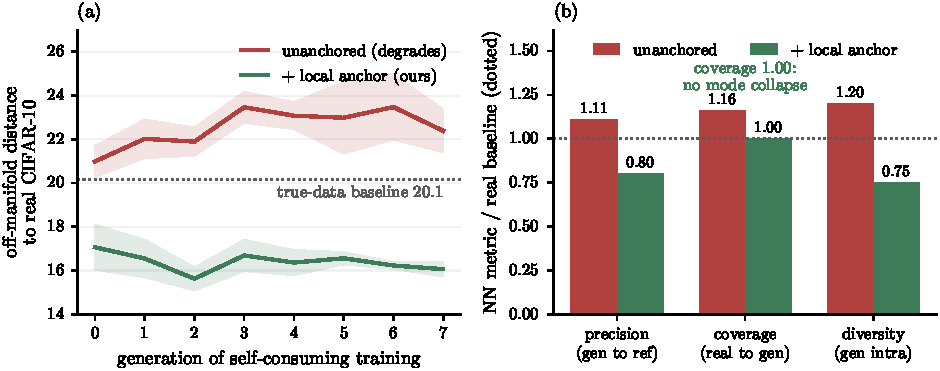
\includegraphics[width=\linewidth]{figs/fig6_cifar.pdf}
\caption{\textbf{CIFAR-10 pixel recursion (\emph{we observe}).} (a) Off-manifold distance
(mean nearest-neighbor distance to held-out real CIFAR-10) across 8 self-consuming
generations, 3 seeds (mean $\pm$ s.d.). The two arms stabilize on opposite sides of the
real-vs-real baseline ($20.1$): unanchored above ($+2.7$, the predicted fattening),
anchored below ($-3.8$, mild contraction toward the manifold); the sign of the split
holds in every seed. Because the two deviations are of comparable size, panel (a) alone
establishes stability, not superiority; the ranking evidence is (b): three
nearest-neighbor metrics relative to a real-vs-real baseline (dotted). The
anchor keeps \emph{coverage} of the real data at $1.00\times$ (no real modes dropped,
ruling out mode collapse) while the unanchored arm loses coverage ($1.16\times$); the
anchor's $0.75\times$ diversity is a bounded, non-compounding
contraction cost (identical at generations 4 and 7).}
\label{fig:cifar}
\end{figure}

\paragraph{Scaling to CIFAR-10 pixels (\emph{we observe}).} To test whether the mechanism
survives at realistic dimension, we ran the same self-consuming recursion in raw CIFAR-10
pixel space ($32\times32\times3=3{,}072$ dimensions) with a small convolutional denoiser
($\sim$7M parameters, mixed precision, single consumer GPU), $\lambda=\tfrac12$, $G=8$,
three seeds (Figure~\ref{fig:cifar}a). Both arms are stable, and they stabilize on
opposite sides of the real-vs-real baseline ($20.1$): the unanchored recursion settles
\emph{above} it (off-manifold distance $22.8\pm1.2$, a deviation of $+2.7$, the
fattening the theory predicts, same sign in every seed), while the anchored recursion
sits \emph{below} it ($16.3\pm0.7$, a deviation of $-3.8$, mild contraction toward the
manifold reflecting the anchor's known diversity cost). We are explicit about what
panel~(a) can and cannot show: the two deviations are of comparable magnitude, so the
distance metric alone ranks neither arm; it establishes that the anchored dynamics are
stable and non-compounding, not that its samples are closer to the data distribution.
The ranking evidence is Figure~\ref{fig:cifar}b: against a real-vs-real baseline, the
anchored arm keeps \emph{coverage} of the real data at $1.00\times$ (no real modes
dropped, ruling out mode collapse) while the unanchored arm loses coverage
($1.16\times$); the anchored arm's reduced intra-set diversity ($0.75\times$) is a
bounded cost, identical at generations 4 and 7 (non-compounding), whereas the unanchored
arm's coverage loss is the collapse itself. At this model budget the samples are blurry;
this is a check on the collapse \emph{dynamics} and a ruling-out of mode collapse, not a
demonstration of perceptual quality. The unanchored arm reaches a stable displaced fixed
point rather than runaway collapse, exactly as Theorem~\ref{thm:law} predicts at
$\lambda=\tfrac12$, where fresh-data injection pins a finite plateau.

\begin{table}[t]
\centering\small
\caption{Headline numbers (mean $\pm$ s.d.\ over seeds; variance in units of $\sigsq$
except MNIST and CIFAR-10, which report off-manifold distance).}
\label{tab:headline}
\begin{tabular}{llll}
\toprule
Experiment & Arm & Final value & Seeds \\
\midrule
Head-to-head, $G{=}20$ & annealed truncation \citep{khelifa2026recursive} & $9.84\pm1.7$ & 5 \\
 & standard sampler $+$ anchor & $1.01\pm0.02$ & 5 \\
 & jump sampler $+$ anchor & $1.01\pm0.02$ & 5 \\
 & annealed $+$ replay ($m{=}2{,}000$ in-pool) & $8.5\pm1.1$ & 5 \\
\midrule
Critical fraction, $t_0{=}10^{-4}$ & $\lambda=0.02$ (subcritical) & $69\pm16$ at $g_{24}$, rising & 3 \\
 & $\lambda=0.25$ (control) & $16.5\pm2.2$ (plateau) & 3 \\
\midrule
Ablation, fixed $t_0{=}10^{-4}$ & stochastic (noise on) & $10.8$ to $13.2$ & 3 \\
 & deterministic (noise zeroed) & $0$ (point collapse) & 3 \\
\midrule
Pixel MNIST, $G{=}8$ & unanchored & $3.06$ & 3 \\
 & anchored & $1.66$ & 3 \\
 & true-data baseline & $1.34$ & n/a \\
\midrule
Pixel CIFAR-10, $G{=}8$ & unanchored & $22.8\pm1.2$ & 3 \\
 & anchored & $16.3\pm0.7$ & 3 \\
 & true-data baseline & $20.1$ & n/a \\
 & anchored coverage / diversity & $1.00\times$ / $0.75\times$ & 3 \\
\midrule
Floor law & envelope bound at measured $\kb{=}3.9$ & $3.8$ (${\sim}60\%$ of measured $6.3$--$7.5$) & n/a \\
 & interventional test, $\kb\!:3.5\to7.5$ & floor $7.6\to\{2.5$--$4.9\}$, above bound & 3 \\
\bottomrule
\end{tabular}
\end{table}

% ================================================================ 8 limitations
\section{Limitations and scope}\label{sec:limits}

Everything in the \emph{we model} tier is collected here. None of it touches the paper's
unconditional core: the closed-form floor (Theorem~\ref{thm:floor}) and the
$\Omega(\sqrt J)$ capacity requirement (Corollary~\ref{cor:capacity}) hold given only the
slope cap $\kb<\infty$, and the memorylessness theorem (Theorem~\ref{thm:fix}) holds given
the frame-cancellation lemma; the items below concern how tightly our \emph{measured}
constants pin the recursion's plateau, not whether the floor exists. Item~(8) is of a
different kind: it delimits which architectures satisfy the slope-cap hypothesis in a
binding way, without bearing on the theorem itself.
(1)~Assumptions~\ref{ass:a0} and~\ref{ass:a2} are measured, cross-validated laws about the
trained pipeline, not derived facts; we present them as such, in the spirit of measured
critical exponents.
(2)~The recursion floor constant is accounted for empirically, not derived: our closed
forms are exact for a single pass and lower bounds for the recursion; feeding the
measured capacity degradation $\kb(w)$ back self-consistently closes a quarter to a
half (in log) of the once factor-$2.4$ gap, and directly measuring the per-pass map's
two remaining channels (in-band profile sag; ensemble displacement) closes it to
$1.1$--$1.3\times$ (Section~\ref{sec:floor}), the level of protocol differences. Every
step of this accounting is a measurement; none of the constants ($\kb$, its
degradation law --- an empirical fit replicated across four synthetic geometries and
real MNIST $8\times8$ pixel data --- or the saturation profile) is derived.
(3)~The residual-field ($\sim30\%$ single-pass) channel is bounded in a
block-correlation model (Appendix~\ref{app:residual}); negative association across
blocks is the one direction that could weaken that particular bound (the closed-form
floor of Theorem~\ref{thm:floor} does not depend on it).
(4)~Curvature is carried at order $O(s^2/\tau)$ in the flat-tube idealization; sphere
experiments bound the resulting bias empirically (non-compounding), but we do not
compute the constants.
(5)~The anchor controls normal \emph{second moments}; tails and tangential statistics
improve but are not anchored; on strongly curved data the anchored recursion shows a
mild residual creep (Figure~\ref{fig:mnist}).
(6)~A parameter-free one-step prediction of MNIST-latent thin ratios fails
quantitatively (it predicts the direction and the regime boundary, not the number); we
flag it rather than fit it.
(7)~Our evidence spans a ring, curved 2-manifolds swept across ambient dimension
$d=8\to128$, six $(t_0,\lambda)$ law-identification cells, the two-horned ablation,
a replay-buffer control and a subcritical-fraction run,
pixel-space MNIST, and a preliminary CIFAR-10 pixel-space recursion ($3{,}072$ dimensions,
three seeds), all chosen so that every quantity the theory names is directly measurable. The
CIFAR-10 run confirms the collapse \emph{dynamics} and rules out mode collapse at scale
(Figure~\ref{fig:cifar}), but at this model budget the samples are blurry and we do not
claim a perceptual-quality result; we do not test latent-diffusion pipelines or
larger models. The theory predicts the mechanism transfers, because the floor depends only
on the \emph{local} normal slope and not on the ambient dimension (Lemma~\ref{lem:frames},
and the measured $d$-independence of the matched floors); confirming this in a large
latent-diffusion system is the clearest next step and is left as future work.
(8)~\textbf{Architectures that factor out the singular normal factor.} The floor's
hypothesis is that the learned normal slope is bounded, $\hat\kappa\le\kb$, which binds
when the network must itself represent the steep normal response. It does \emph{not} bind
for parameterizations that build the singular factor into the sampler by construction, for
instance a score of the form $-(x-\hat x)/h(t)$ with a learned projection-like map $\hat x$,
as in the SiLD construction of \citet{huang2026provable}: there the network supplies
$\hat x$ rather than the slope, and $\hat\kappa$ is not limited by network capacity.
Theorem~\ref{thm:floor} is silent about such models. The experiments here all use ordinary
$\eps$-prediction, for which the hypothesis does bind. We thank Wei Huang for this
observation. The finite-capacity question does not disappear in that setting, it relocates:
writing $\hat x=\Pi_M(x)+\delta(x)$, the score error carries a term of order
$\delta(x)/h(t)$, so projection error is amplified by the same singular factor as $t\to0$.
Whether that amplification admits a floor of the same $\kb^{-2}$ character, with
$\E[\delta^2]$ in place of the slope deficit, is open and is the clearest theoretical
extension of this work.

\section{Reproducibility}\label{sec:repro}

Code, result logs, and figures are public at\\
\centerline{\url{https://github.com/Naman84789/model-collapse-manifolds}}\\
Every claim maps to a script, an append-only result log, and a figure in the released
code (ring, ablation, replay and critical-fraction controls, MNIST, floor law, law
identification; $\sim$3 CPU-hours total).
The result figures regenerate from logged data in seconds. A README lists the
run order, the load-bearing scripts, and the headline numbers a reproduction
must match. The released code also includes an adversarial verification script for
Theorem~\ref{thm:floor}: it re-derives the band crossing symbolically (independent of the
manuscript's derivation), integrates the limit ODE with an independent solver, confirms
the limiting cases $\rho\to0$, $\rho\to1^-$, $\kb\to\infty$, and $\lambda\to1$, verifies
that the boundary layer contracts at the predicted quadratic rate, and attacks the
comparison bound with 200 randomized slope profiles including overshooting ones; all
checks pass.

\subsubsection*{Acknowledgments}
Numerical experiments, figure preparation, and portions of the derivations were carried
out with the assistance of an AI system (Claude, Anthropic), used as a research tool
under the author's direction; the author reviewed all mathematics and takes full
responsibility for every claim.

\bibliographystyle{unsrtnat}
\bibliography{refs}

\clearpage
\appendix

% ================================================================ A proofs law
\section{Proof of Theorem~\ref{thm:law}}\label{app:law}

Write $h(v):=T(v)-v$ with $T$ as in \eqref{eq:recursion} (we reserve $g$ for the
generation index); $h$ is concave (composition of
an affine map with the concave nondecreasing $w\mapsto w+e^2(w)$, minus a linear term),
with $h(0)=T(0)=\lambda\sigsq+e^2(\lambda\sigsq)>0$ and one-sided derivative
$h'(v)=(1-\lambda)\big(1+e^{2\prime}(w(v))\big)-1$, nonincreasing in $v$ with limit
$(1-\lambda)(1+c_\infty)-1<0$ when $\lambda>\lambda^*$.

\textbf{(i) Existence, uniqueness.} A concave function positive at $0$ whose derivative
is eventually $\le-\delta<0$ tends to $-\infty$, so $h$ has a zero; concavity plus
$h(0)>0$ forbids two downcrossings, so the zero $v_\infty$ is unique, with $T(v)>v$ for
$v<v_\infty$ and $T(v)<v$ for $v>v_\infty$.

\textbf{Contraction above.} For $v\ge v_\infty$, monotonicity and concavity give
$0\le T(v)-v_\infty\le\rho_{\mathrm{loc}}(v-v_\infty)$ with
$\rho_{\mathrm{loc}}=T'(v_\infty^+)<1$. The strict inequality needs no extra
hypothesis: if $\rho_{\mathrm{loc}}=1$ then $h'(v_\infty)=0$, making the concave $h$
maximal at $v_\infty$, whence $h(v_\infty)\ge h(0)=T(0)>0$, contradicting
$h(v_\infty)=0$. So the crossing is always strict and the rate genuinely geometric.

\textbf{Convergence under vanishing perturbations.} Let $v_g=T(v_{g-1})+s^2_g$,
$s^2_g\to0$. While iterates stay $\ge v_\infty$,
$x_g:=v_g-v_\infty\le\rho_{\mathrm{loc}}x_{g-1}+s^2_g\to0$ by the standard perturbed
contraction argument (split $\sum_j\rho_{\mathrm{loc}}^{\,g-j}s^2_j$ at $j=g/2$). If an iterate drops
below $v_\infty$: define the unperturbed comparison $u_g=T(u_{g-1})$ started there; then
$u_g\uparrow v_\infty$ (monotone, bounded, $T(v)>v$ below $v_\infty$) and $v_g\ge u_g$ by
induction ($s^2_g\ge0$, $T$ monotone), so $\liminf v_g\ge v_\infty$, while
$v_g<v_\infty+s^2_g$ gives $\limsup v_g\le v_\infty$. Alternating regimes inherit both
barriers. Linearizing $T$ at $v_\infty$ gives the local rate.

\textbf{(ii) Divergence.} If $(1-\lambda)(1+c_\infty)>1$ then, since $e^{2\prime}\ge
c_\infty$ everywhere (the concave derivative decreases \emph{to} its limit), $h'\ge
(1-\lambda)(1+c_\infty)-1>0$, so $h$ is nondecreasing and $h(v)\ge h(0)>0$ for all $v$:
after $G$ generations $v_G\ge v_0+G\,T(0)\to\infty$, regardless of the schedule
($s^2_g\ge0$ only helps).

\textbf{(iii)} Substituting $e^2(w)=e_0^2+cw$ makes $T$ affine with slope
$(1+c)(1-\lambda)$; solve the fixed point. \qed

% ================================================================ B variance ODE
\section{The variance ODE}\label{app:ode}

\textbf{Lemma~\ref{lem:ode}.} One Euler step of the reverse scheme is
$x'=x+\big(\tfrac12x-\epshat(x,t)/s\big)dt+\sqrt{dt}\,\xi$ with $\xi$ independent of $x$.
Write $f(x)=\tfrac12x-\epshat(x,t)/s$. By bilinearity of the covariance and independence of
the injected noise,
\[
\Var(x')=\Var(x)+2\,dt\,\Cov\big(x,f(x)\big)+dt^2\Var\big(f(x)\big)+dt
=V+\Big[V-\tfrac{2}{s}\Cov\big(x,\epshat(x)\big)+1\Big]dt+O(dt^2).
\]
No property of $\epshat$ beyond square-integrability is used, so this holds for a
nonlinear estimator; the $+dt$ is the injected noise and the $O(dt^2)$ term is the finite
variance of the drift. Divide by $dt$, let $dt\to0$, and substitute
$\Cov(x,\epshat(x))=\hat\kappa\Var(x)$ from \eqref{eq:khat} to get \eqref{eq:varode}.

\emph{Independent route, no discretisation.} For the continuous reverse SDE
$dX=f(X)d\tau+dW$, It\^o gives $d(X^2)=2Xf(X)d\tau+2X\,dW+d\tau$, so
$\E[X^2]'=2\E[Xf(X)]+1$ while $\E[X]'=\E[f(X)]$; subtracting,
$\Var'=2\Cov\big(X,f(X)\big)+1$, which is \eqref{eq:varode}. With $\hat\kappa=\kappa=s/\gamma^2$: $\kappa/s=1/\gamma^2$ and
$V=\gamma^2$ solves the equation exactly (direct check), confirming the bookkeeping. An
intercept in $\epshat$ moves only the mean. \qed

\textbf{Remark~\ref{rem:lip}.} For an i.i.d.\ copy $X'$ of $X$,
$\tfrac12\E[(X-X')(g(X)-g(X'))]$ expands to $\E[Xg(X)]-\E[X]\E[g(X)]=\Cov(X,g(X))$. If $g$
is $\kb$-Lipschitz then $(X-X')(g(X)-g(X'))\le\kb(X-X')^2$ pointwise, and
$\E[(X-X')^2]=2\Var(X)$, so $\Cov(X,g(X))\le\kb\Var(X)$ under any law. \qed

% ================================================================ C floor proofs
\section{Floor lemmas and closed forms}\label{app:floor}

\textbf{Lemma~\ref{lem:band}.} From \eqref{eq:kappa}, $\kappa(t)=s/(a^2\sigsq+s^2)$
with $s^2=1-e^{-t}$: $\kappa\to0$ as $t\to0$ ($s\to0$, $\gamma^2\to\sigsq$),
$\kappa\approx1/s$ for $s^2\gg\sigsq$, and maximizing over $s$ gives
$\kappa_{\max}=1/(2\sigma)$ at $s=\sigma$ (i.e.\ $t\approx\sigsq$), to leading order in
$\sigsq$. Below the band the remaining e-folds are
$\int_{t_0}^{t_-}2\kappa/s\,dt=\int 2\,dt/\gamma^2=2\log\frac{\sigsq+t_-}{\sigsq+t_0}
\le2\log(1+\rho^2/4)\le\rho^2/2$, using $t_-\approx\kb^2\sigma^4$. \qed

\textbf{Lemma~\ref{lem:limitode}.} Substitute $t=\sigsq u$, $V=\sigsq W$:
$s^2=\sigsq u(1+O(\sigsq u))$, $\gamma^2=\sigsq(1+u)(1+O(\sigsq u))$, so
$\kappa=(1/\sigma)\frac{\sqrt u}{1+u}(1+O(\sigsq u))$ and
$2\hat\kappa/s=(2m(u)/\sqrt u)/\sigsq$; the ODE becomes
$-dW/du=1-(2m/\sqrt u)W+\sigsq W(1+o(1))$. On $u\in[0,U]$ the perturbing terms are
$O(\sigsq U)$ \emph{per unit of} $W$; the band occupies $u\le u_+=O(1/\rho^2)$, giving
the stated \emph{relative} error $O(\sigsq/\rho^2)$ (the additive gap to $g$ is a factor
$W\sim\rho^{-2}$ larger, hence $O(\sigsq/\rho^4)$). For the boundary: the uncapped equation
$-dW/du=1-2W/(1+u)$ has general solution $W=(1+u)+A(1+u)^2$ (direct check), so
deviations from the slave solution $W=1+u$ contract as $\big((1+u)/(1+u')\big)^2$ under
downward integration from $u'$ to $u$; the influence of the $t\gtrsim1$ boundary layer
at band entry is suppressed by this quadratic factor and is absorbed in the same error
term. \emph{Numerical check:} the slave solution is invariant to $3\times10^{-15}$ under
the integrator; finite-$\sigma$ floors converge to the limit values from above
(e.g.\ $\rho=0.39$: $3.953/3.812/3.775$ at $\sigma=0.10/0.05/0.02$ vs.\ limit $3.769$).
\qed

\textbf{Theorem~\ref{thm:floor}(U).} By the scalar comparison principle
(equal forcing and data; smaller $\hat\kappa$ means larger $V$), any profile with
$\hat\kappa\le\kb$ has $V\ge V_{\hat\kappa\equiv\kb}$, one-sided; no lower bound on
$\hat\kappa$ is used. For the constant envelope, \eqref{eq:limitode} with
$m\equiv\rho/2$ has integrating factor $e^{-2\rho\sqrt u}$:
$\frac{d}{du}\big[We^{-2\rho\sqrt u}\big]=-e^{-2\rho\sqrt u}$, so for data of
sub-quadratic growth at $u=\infty$,
$W(0^+)=\int_0^\infty e^{-2\rho\sqrt u}du=2\int_0^\infty xe^{-2\rho x}dx=\frac1{2\rho^2}$,
exactly, for every $\rho>0$. $1/(2\rho^2)>1\iff\rho<1/\sqrt2$.

\textbf{Theorem~\ref{thm:floor}(N).} The band edges solve $\sqrt u/(1+u)=\rho/2$, a
quadratic in $x=\sqrt u$: $\rho x^2-2x+\rho=0$, $x_\mp=(1\mp q)/\rho$, $q=\sqrt{1-\rho^2}$
(nonempty iff $\rho<1$). Above the band the solution is the exact slave $W=1+u$; it
enters the band with $W(u_+)=1+u_+$. Across the band ($m=\rho/2$), the same integrating
factor with antiderivative $F(u)=-(2\rho\sqrt u+1)e^{-2\rho\sqrt u}/(2\rho^2)$ gives
\[
W(u_-)=(1+u_+)e^{-2\rho(x_+-x_-)}
+\frac{(2\rho x_-+1)-(2\rho x_++1)e^{-2\rho(x_+-x_-)}}{2\rho^2},
\]
and $2\rho x_\mp=2(1\mp q)$, $2\rho(x_+-x_-)=4q$ yield the displayed $W_{\mathrm{exit}}$.
Below the band the equation is uncapped with exact general solution $(1+u)+A(1+u)^2$;
matching at $u_-$ gives $A=\big(W(u_-)-(1+u_-)\big)/(1+u_-)^2$ and
$g(\rho)=W(0^+)=1+A$, which is \eqref{eq:closedform}. Limits: as $\rho\to1^-$ ($q\to0$),
$u_\pm\to1$ and $g\to1$; as $\rho\to0$ ($q\to1$), $u_+\approx4/\rho^2$,
$u_-\approx\rho^2/4$, and expanding,
$g=\big[8e^{-4}+1-5e^{-4}\big]/(2\rho^2)+O(1)=(1+3e^{-4})/(2\rho^2)+O(1)$, giving
$C_0=(1+3e^{-4})/2$. Positivity $g>1$ on $(0,1)$ follows from $W(u_-)>1+u_-$ (the band
under-contracts relative to the slave). \emph{Numerical check:} \eqref{eq:closedform}
and the exact $1/(2\rho^2)$ match direct integration of \eqref{eq:limitode} to
$\le2.4\times10^{-5}$ over $\rho\in[0.1,1]$ (pure Euler residual).

Both bounds apply to the fully nonlinear estimator with no extension step, since
\eqref{eq:varode} is exact and $\hat\kappa$ is defined under the sampler's own law
(Lemma~\ref{lem:ode}). Lemma~\ref{lem:limitode} transfers the
limit values to finite $\sigma$ with the stated error. \qed

\textbf{Corollary~\ref{cor:capacity}} is Theorem~\ref{thm:floor}(U) read at fixed
$\kb$ with $\sigma\to0$; the capacity bound inverts $1/(2\rho^2)\le C$. \qed

% ================================================================ D sharpening
\section{Posterior-mean sharpening and per-axis necessity}\label{app:sharpening}

\begin{proposition}[Tweedie sharpening; \emph{we prove}]\label{prop:sharpening}
In the Gaussian normal coordinate with axis variance $\sigma^2_{\mathrm{ax}}$, the jump
with the exact predictor outputs the posterior mean, with
\[
\Var(\hat x_0)=\frac{a^2\sigma^4_{\mathrm{ax}}}{\gamma^2_{\mathrm{ax}}(\hat t)},\qquad
\frac{\Var(\hat x_0)}{\sigma^2_{\mathrm{ax}}}
=\frac{a^2\sigma^2_{\mathrm{ax}}}{a^2\sigma^2_{\mathrm{ax}}+s^2(\hat t)}<1 ,
\]
and with a trained predictor $\epshat=\eps^*-\tilde\delta$,
$v_{\mathrm{jump,ax}}=a^2\sigma^4_{\mathrm{ax}}/\gamma^2_{\mathrm{ax}}
+(s^2/a^2)\E[\tilde\delta^2]+2(s/a)\,\mathrm{Cov}+O(s^4/\tau^2)$.
\end{proposition}

\begin{proof}
$\hat x_0=(x-s\eps^*)/a=x(1-s^2/\gamma^2)/a=(a\sigma^2_{\mathrm{ax}}/\gamma^2)x$, so
$\Var=a^2\sigma^4_{\mathrm{ax}}/\gamma^2$; Tweedie's formula identifies this with
$\E[X_0\,|\,X_{\hat t}]$ \citep{efron2011tweedie}. The error term is the jump map
applied to $\eps^*-\tilde\delta$; the curvature term is the posterior-mean chord bias.
\end{proof}

Consequences: strongly singular axes ($\sigma_{\mathrm{ax}}\ll s$) are collapsed onto
the manifold (the matcher must top up); fat axes ($\sigma_{\mathrm{ax}}\gg s$) are
untouched while injection fattens them (the matcher must contract); axes with
$\sigma_{\mathrm{ax}}\sim s$ sharpen by an axis-dependent factor strictly inside
$(0,1)$. Hence the required correction is signed and anisotropic: any correct matcher
must be bidirectional and per-axis. (\emph{We observe:} scalar matching leaves
thin ratios at $0.62$ to $0.65$ on MNIST latents; per-axis matching achieves
$|\text{thin}-1|\le0.012$.)

% ================================================================ E residual
\section{The residual channel (\emph{we model})}\label{app:residual}

(\emph{Role revised by measurement}: the floor anatomy of Section~\ref{sec:floor}
identifies the single-pass remainder beyond the envelope as two measured channels ---
in-band profile sag and the deterministic ensemble-displacement effect --- with the
residual beyond them small and slightly negative; this appendix's stochastic bound is
retained as a consistency check on the residual field's magnitude, not as the
remainder's explanation.)

The residual of the estimator about its affine $L^2(p_t)$ fit,
$\delta:=\epshat-\hat\kappa_{\mathrm{aff}}x-b$ (used in this appendix only, as an
independent characterisation of the residual field; the floor proof does not rely on it),
has measured band risk
$r^2_{\mathrm{res}}(t)\approx0.02$ to $0.05$, flat in $t$ and in sample size, with
path-coherence time $\approx\nu t$, $\nu\approx0.75$. Under a block-correlation model
(coherent within blocks of length $\nu t$, independent across blocks, no systematic
over-contraction), the injected variance obeys
$\Phi_0(t_0)\ge c\,\nu\rho_0(\sigsq+t_0)$: decreasing in $t_0$ until $t_0\sim\sigsq$,
then saturating, the same shape as the measured excess (knee at $t_0\approx\sigsq$,
$n$-flat), with the single constant effective to within a factor $\sim2$. In this paper
the channel plays a supporting role only: it is the measured $\sim30\%$ single-pass
remainder on top of the closed-form floor, which does not depend on it.

% ================================================================ F protocols
\section{Experimental details}\label{app:details}

\textbf{Networks and training.} 3-layer MLPs, width 256, SiLU, 32-dim sinusoidal time
embedding; Adam, learning rate $2\times10^{-3}$; batch 512 (ring) / 256 (MNIST);
denoising score matching with $t\sim U(10^{-3},8)$; fresh network each generation.

\textbf{Sampling.} Reverse Euler-Maruyama on a 200-point geometric grid from $T=8$;
the ablation zeroes the $\sqrt{|dt|}\,\xi$ term only. Jump: $\hat t=0.05$.

\textbf{Anchor.} Ring: radial (normal) bidirectional match of the pool's radial
variance to the stale reference's, contract-by-scaling / top-up-by-noise. MNIST:
per-point $k$NN-PCA ($k=96$, $k_{\dim}=12$) charts from the reference; normal
coordinates rescaled to the reference's local normal eigenvalues in the same frames.
Reference: $m=2{,}000$ real samples drawn once at $g=0$, never refreshed
(provenance-free: the matcher is applied to the whole pool without labels).

\textbf{Measured network profile.} The fitted slope $\hat\kappa(t)$ is extracted by
affine regression of $\epshat$ against $x$ on fiber lines at each $t$; it tracks
$\kappa(t)$ ($0.95$ to $0.97$ for $t\ge0.1$), saturates at $\kb\approx3.9$ inside the
band, and never exceeds $\kappa$ ($n$-independent across $1$k to $16$k) --- a
data-width statement: nets trained on fat pools ($\sqrt w\gtrsim0.10$) show mild
overshoot at mid times, so the class-(N) constant applies at the data width while
class (U) needs no such assumption. The decomposition
identity $(\kappa-\hat\kappa)^2\gamma^2+r^2_{\mathrm{res}}=r^2_{\mathrm{tot}}$ checks
numerically along the path.

\textbf{$t_0$-dependence of the response slope.} The probe's net slope
$c\in\{0.00,\dots,0.13\}$ is measured at its sampling point $t_0=5\times10^{-3}$. At
the recursion's operating point $t_0=10^{-4}$, the directly measured per-pass map over
the same widths has $dv/dw\approx0.68$ ($c\approx-0.32$): once the sampler traverses
the whole band, the deficit channel dominates and $e^2$ \emph{decreases} over this
range --- still within the law's requirement ($e^{2\prime}>-1$ keeps $T$ monotone and
concave, and only strengthens contraction), and consistent with the plateau
measurements ($e^2(w^*)=3.9$--$5.0\,\sigsq$ falling with the fixed point's width). The
$\lambda=0.02$ runaway then implies the slope turns back positive in the far-fat
regime ($w\gg10\,\sigsq$), outside the anatomy's measured range; Assumption~\ref{ass:a2}'s
global nondecreasing-concave form is a regime model, exact where identified.

\textbf{Anatomy of $c$.} Training single-width tubes at
$w\in\{0.0009,\dots,0.0169\}$ and measuring $dv/dw-1$ gives net
$c\in\{0.00,0.05,0.13,0.10,0.05\}$ (small, positive, concave) as the sum of a
deficit response $\approx-0.68$ (a fatter pool needs a smaller peak slope) and an
injection response $\approx+0.73$ (a fatter pool damps injected variance less).
The same probe's per-width slope fits give the capacity-degradation fit
$\kb(w)=4.43-11.6\sqrt{w}$ used in Section~\ref{sec:floor}, which refines this
anatomy into three channels: writing
$\tfrac{d}{dw}\Phidet(w,\kb(w))
=\partial_w\Phidet|_{\kb}+(\partial_{\kb}\Phidet)\,\kb'(w)$, the mid-range values
are a deficit $\approx-0.94$ and a capacity-degradation term $\approx+0.7$
(the latter is not a fit artifact: raw centered differences of the five measured
points, with no functional form at all, give $+0.78/+0.68/+0.67$ at the three
interior widths vs.\ the fit's $+0.84/+0.70/+0.65$). The derived deterministic
response is therefore $\approx-0.23$ mid-range, and the measured total ($+0.10$
to $+0.13$) leaves a residual attributed to injection of $\approx+0.3$ to
$+0.4$. Because injection is \emph{defined} as this residual, the three channels
sum to the measurement by construction; the non-trivial content is that the
residual comes out stable, positive, and of the size the residual-channel model
(Appendix~\ref{app:residual}) expects, and that most of what the two-channel
anatomy above attributes to injection is really $\kb$ degrading on fatter pools.
We trust the split mid-range only: at the thinnest width $\kb'(w)$ from the
$\sqrt w$ fit diverges, an artifact of the parametrization, not a mechanism.

\end{document}
